\section{Preliminary results}\label{sec:results}

\revised{This section reports our results.
\Cref{sec:evaluation,sec:market-rent,sec:errors,sec:drivers,sec:concessions,sec:pipeline} cover the
synthetic data, where the truth layer lets us score predictions against the true market rent.
\Cref{sec:real-results} gives our first results on the real Chicago listings.}

\subsection{Evaluation}\label{sec:evaluation}

We evaluate every model on buildings it has never seen. Listings are split by building,
\nTrainBuildings{} for training and \nTestBuildings{} for testing, so no building contributes to
both. With about \listingsPerBuilding{} listings per building, a split by listing would let a model
memorize buildings and overstate its accuracy. Our primary metric is the median absolute percentage
error,
\[
  \mathrm{MdAPE} \;=\; \operatorname*{median}_{i}\, \frac{\lvert \hat{y}_i - y_i \rvert}{y_i},
\]
which reads directly as a typical miss, compares fairly across markets with different rent levels,
and is not dominated by the few luxury units with the largest dollar errors. We also report the mean
absolute error (MAE) in dollars and \(R^2\). \revised{We also score} each model twice: against the
asking rent it was trained to predict, and against the generator's true market rent for the same
floor plan and month, a comparison that only synthetic data allows. \revised{On the real Chicago
data, models are evaluated on held-out rental units. That data has no truth layer, so we compare
models by MAE, \(R^2\), and the root mean squared error (RMSE), which penalizes large misses more
heavily. We will add MdAPE so that the two datasets can be compared directly.}

\subsection{Market rent}\label{sec:market-rent}

\Cref{tab:models} compares the three models with the naive baseline. Gradient boosting performs
best, cutting the baseline's median error by \errorReduction{}, from \baseMdape{} to \gbmMdape{}, with
an MAE of \gbmMae{} and an \(R^2\) of \gbmRsq{} on the \nTestListings{} listings of the held-out
buildings. It also lowers MAE by \gbmVsLinear{} compared with linear regression. Because the data
are synthetic and a single test set was used to compare the models, these results are a working
baseline rather than a model selection.

The last row of \cref{tab:models} is the most informative. A listing's own asking rent sits within
\noiseFloor{} of the true market rent, which means asking rent is a reliable training target, and
each model's error against the true rent (\gbmMdapeTrue{} for gradient boosting) matches its error
against the asking rent. The remaining error therefore does not come from noise in the listings. It
comes from information about each building that our \nFeatures{} variables do not capture.
\revised{Nearby comparable buildings carry that information, which is why comparable-property selection
is our next step.}

\begin{table}[htbp]
  \caption{Performance on \nTestBuildings{} held-out buildings (\nTestListings{} listings). MdAPE is
  measured against each listing's asking rent and against the generator's true market rent for its
  floor plan and month. The last row is how far the listing itself sits from the truth.}
  \label{tab:models}
  \centering\small
  \begin{tabular}{@{}l S[table-format=3.0] S[table-format=1.2] S[table-format=2.1] S[table-format=2.1]@{}}
\toprule
 & {MAE} & {\(R^2\)} & \multicolumn{2}{c}{MdAPE (\%)} \\
\cmidrule(l){4-5}
Model & {(\$)} & & {vs.\ asking} & {vs.\ true} \\
\midrule
Naive baseline (market \(\times\) bedrooms median) & 443 & 0.30 & 21.0 & 21.0 \\
Linear regression & 285 & 0.70 & 13.0 & 13.1 \\
Decision tree & 302 & 0.65 & 13.3 & 13.2 \\
\textbf{Gradient boosting} & 235 & 0.79 & 10.6 & 10.6 \\
\midrule
The listing's own asking rent & {---} & {---} & {---} & 2.8 \\
\bottomrule
\end{tabular}

\end{table}

\begin{figure}[htbp]
  \centering
  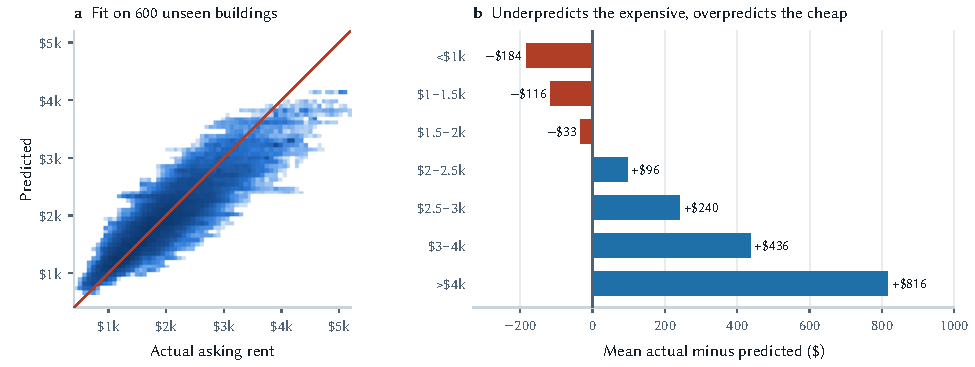
\includegraphics{fit}
  \caption{Predictions on held-out buildings. (a)~Each square is a bin of listings, darker where more
  fall; the red line is perfect prediction. (b)~Mean error by actual rent: the model pulls toward the
  middle, overpredicting the cheapest units by \biasLow{} and underpredicting the most expensive by
  \biasHigh{}.}
  \label{fig:fit}
\end{figure}

\subsection{Where the model errs}\label{sec:errors}

Errors grow with rent (\cref{fig:fit}). The model pulls its predictions toward the middle: low rents
are overpredicted and high rents underpredicted, by an average of \biasLow{} for units under \$1,000
and \biasHigh{} for units above \$4,000. \Cref{fig:segments} breaks the error down by segment. It is
largest for class C buildings and for units with four or more bedrooms, and the bias differs by
property class: class A buildings are underpredicted and class C buildings overpredicted. This
pattern is consistent with the model not yet using property class, the strongest categorical
variable we identified. Lease-up buildings, which we expected to be harder, are in fact predicted
slightly better than stabilized ones (\mdapeLeaseUp{} against \mdapeStabilized{}).

\begin{figure}[htbp]
  \centering
  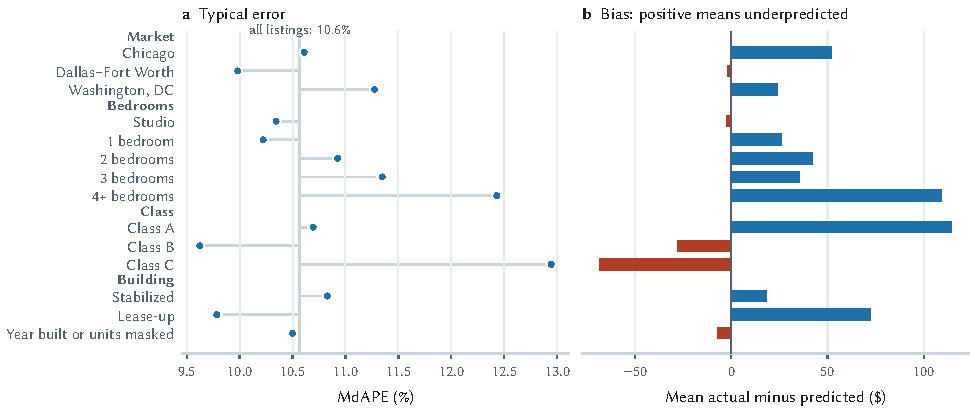
\includegraphics{segments}
  \caption{Error by segment on held-out buildings. (a)~MdAPE; the vertical line is the overall
  \gbmMdape{}. (b)~Mean actual minus predicted rent. Class A is underpredicted and class C
  overpredicted, consistent with the model lacking property class, the strongest categorical
  candidate in \cref{fig:drivers}.}
  \label{fig:segments}
\end{figure}

\subsection{What drives the predictions}\label{sec:drivers}

\Cref{fig:drivers}a shows how much each input contributes on unseen buildings, measured by the
increase in MAE when that input is shuffled. Unit size matters most, adding \topFeatureDmae{} to the
MAE when shuffled, followed by latitude, the building's amenity count, and longitude. Location ranks
high in this test, consistent with our exploratory analysis, while bathrooms and the number of units
sharing the floor plan add almost nothing once the other inputs are known. \Cref{fig:drivers}b and~c
show why we select categorical variables on held-out importance rather than in-sample fit: state and
metro area fit the training buildings well but add nothing on unseen ones, while property class is
by far the most useful.

\begin{figure}[htbp]
  \centering
  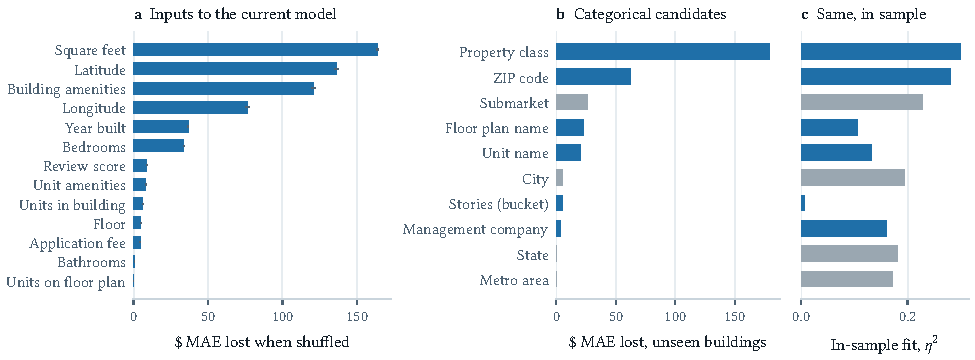
\includegraphics{drivers}
  \caption{Which inputs matter on unseen buildings. (a)~Dollars of mean absolute error added when
  each of the model's \nFeatures{} inputs is shuffled. (b)~The same measure for the categorical
  candidates, blue where kept. (c)~Their in-sample fit: state and metro area fit the training
  buildings but add nothing on unseen ones.}
  \label{fig:drivers}
\end{figure}

\subsection{Concession extraction}\label{sec:concessions}

The extractor gets the amount right for \concAmountAcc{} of the \concN{} specials that state their
terms, and values the concession within 5\% for \concWithinFive{} of them (\cref{fig:concessions}, in
\cref{app:figures}).
Accuracy depends on how the text was written. On specials written by a language model the rules are
right \concLlm{} of the time, but on the generator's template text they are right only \concGrammar{}
of the time, because these specials often quote a dollar amount or a net effective rent where the
truth layer records months free. Every dollar-denominated special is read correctly, while specials
offering free months reach \concMonthsFree{}.


\subsection{Pipeline and reproducibility}\label{sec:pipeline}

All of our code and outputs are shared through the team's GitHub repository. Three commands rebuild
the master table from the public download, and 59 join checks verify that the merged table is
complete and consistent. \revised{The same code recomputes every
synthetic-data number, table, and figure in this report from the data, so the report stays
consistent with the models behind it.}


\subsection{Preliminary results on real Dwellsy data}\label{sec:real-results}

\revised{\Cref{tab:real-models} compares the five models on the Chicago validation set.}

\begin{table}[htbp]
  \caption{\revised{Preliminary performance on real Chicago listings, measured on the validation set
  (rental units held out from training).}}
  \label{tab:real-models}
  \centering\small
  \revised{\begin{tabular}{@{}lrrr@{}}
    \toprule
    Model & MAE (\$) & RMSE (\$) & \(R^2\) \\
    \midrule
    \textbf{Gradient boosting} & 229 & 396 & 0.83 \\
    Random forest & 291 & 465 & 0.77 \\
    Linear regression & 335 & 552 & 0.68 \\
    Decision tree & 346 & 533 & 0.70 \\
    Baseline (mean training rent) & 669 & 970 & 0.00 \\
    \bottomrule
  \end{tabular}}
\end{table}

\revised{Gradient boosting performs best, with an MAE of \$229 and an \(R^2\) of 0.83, against \$669 and
0.00 for the baseline. As on the synthetic data, it beats linear regression and a single decision
tree, and the random forest comes second. The two tree ensembles outperform the simpler models,
which suggests that rent depends on interactions between unit characteristics and location. We will
tune these models and test others before choosing one.}

\revised{The Ridge regression tests whether exact location adds information beyond ZIP code. Adding spline
transformations of latitude and longitude lowered validation MAE by only \$1.78 and raised \(R^2\) by
0.0024, so in this model ZIP code already captures most of the location signal.}
